\documentclass[a4paper]{article}\usepackage{graphicx, color}
%% maxwidth is the original width if it is less than linewidth
%% otherwise use linewidth (to make sure the graphics do not exceed the margin)
\makeatletter
\def\maxwidth{ %
  \ifdim\Gin@nat@width>\linewidth
    \linewidth
  \else
    \Gin@nat@width
  \fi
}
\makeatother

\definecolor{fgcolor}{rgb}{0.2, 0.2, 0.2}
\newcommand{\hlnumber}[1]{\textcolor[rgb]{0,0,0}{#1}}%
\newcommand{\hlfunctioncall}[1]{\textcolor[rgb]{0.501960784313725,0,0.329411764705882}{\textbf{#1}}}%
\newcommand{\hlstring}[1]{\textcolor[rgb]{0.6,0.6,1}{#1}}%
\newcommand{\hlkeyword}[1]{\textcolor[rgb]{0,0,0}{\textbf{#1}}}%
\newcommand{\hlargument}[1]{\textcolor[rgb]{0.690196078431373,0.250980392156863,0.0196078431372549}{#1}}%
\newcommand{\hlcomment}[1]{\textcolor[rgb]{0.180392156862745,0.6,0.341176470588235}{#1}}%
\newcommand{\hlroxygencomment}[1]{\textcolor[rgb]{0.43921568627451,0.47843137254902,0.701960784313725}{#1}}%
\newcommand{\hlformalargs}[1]{\textcolor[rgb]{0.690196078431373,0.250980392156863,0.0196078431372549}{#1}}%
\newcommand{\hleqformalargs}[1]{\textcolor[rgb]{0.690196078431373,0.250980392156863,0.0196078431372549}{#1}}%
\newcommand{\hlassignement}[1]{\textcolor[rgb]{0,0,0}{\textbf{#1}}}%
\newcommand{\hlpackage}[1]{\textcolor[rgb]{0.588235294117647,0.709803921568627,0.145098039215686}{#1}}%
\newcommand{\hlslot}[1]{\textit{#1}}%
\newcommand{\hlsymbol}[1]{\textcolor[rgb]{0,0,0}{#1}}%
\newcommand{\hlprompt}[1]{\textcolor[rgb]{0.2,0.2,0.2}{#1}}%

\usepackage{framed}
\makeatletter
\newenvironment{kframe}{%
 \def\at@end@of@kframe{}%
 \ifinner\ifhmode%
  \def\at@end@of@kframe{\end{minipage}}%
  \begin{minipage}{\columnwidth}%
 \fi\fi%
 \def\FrameCommand##1{\hskip\@totalleftmargin \hskip-\fboxsep
 \colorbox{shadecolor}{##1}\hskip-\fboxsep
     % There is no \\@totalrightmargin, so:
     \hskip-\linewidth \hskip-\@totalleftmargin \hskip\columnwidth}%
 \MakeFramed {\advance\hsize-\width
   \@totalleftmargin\z@ \linewidth\hsize
   \@setminipage}}%
 {\par\unskip\endMakeFramed%
 \at@end@of@kframe}
\makeatother

\definecolor{shadecolor}{rgb}{.97, .97, .97}
\definecolor{messagecolor}{rgb}{0, 0, 0}
\definecolor{warningcolor}{rgb}{1, 0, 1}
\definecolor{errorcolor}{rgb}{1, 0, 0}
\newenvironment{knitrout}{}{} % an empty environment to be redefined in TeX

\usepackage{alltt}


\usepackage{graphicx}
\usepackage{graphics}

\usepackage[english]{babel}
\usepackage[figuresright]{rotating}
\usepackage{bm}

\usepackage{enumerate}
\usepackage{float}
\usepackage{dsfont}

\usepackage{amsmath}
\usepackage{amsfonts}
\usepackage{amssymb}
%\usepackage{natbib}
\usepackage{authblk}

\usepackage{color}
%%%%%%%%%%%%%%%%%%  Author newcommand begin
\newtheorem{defi}{Definition}

\newcommand{\E}{\mathbb{E}}
\newcommand{\R}{\mathbb{R}}
\renewcommand{\P}{\mathbb{P}}
\newcommand{\Var}{\mathbb{V}ar}
\newcommand{\Cov}{\mathbb{C}ov}
\newcommand{\Comb}[2]{\left(\begin{array}{c}#1 \cr #2\end{array}\right) }
%%%%%%%%%%%%%%%%%  Author newcommend end

\usepackage[sc]{mathpazo}
\usepackage[T1]{fontenc}
\usepackage{geometry}
\geometry{verbose,tmargin=2.5cm,bmargin=2.5cm,lmargin=2.5cm,rmargin=2.5cm}
\setcounter{secnumdepth}{2}
\setcounter{tocdepth}{2}
\usepackage{url}
%\usepackage[unicode=true,pdfusetitle,
% bookmarks=true,bookmarksnumbered=true,bookmarksopen=true,bookmarksopenlevel=2,
% breaklinks=false,pdfborder={0 0 1},backref=false,colorlinks=false]
% {hyperref}
%\hypersetup{
% pdfstartview={XYZ null null 1}}
%\usepackage{breakurl}

\usepackage{courier}
%% Newcommand for tuna report
\newcommand{\iscam}{\texttt{iSCAM}}
\newcommand{\admb}{\texttt{admb} }
\newcommand{\com}[1]{\textcolor{red}{#1}}
\title{Report for ICCAT-GBYP 04/2013}
%\author{Marie-Pierre Etienne\thanks{marie.etienne@agroparistech.fr}}
%\author{Tom Carruthers }
%\author{Murdoch McAlllister}
%\affil[1]{AgroParisTech}
%\affil[2]{UBC}
\IfFileExists{upquote.sty}{\usepackage{upquote}}{}

\begin{document}







\maketitle
\section{Introduction}

\verb+admb+ and \verb+iSCAM+ are assumed to be installed, a \verb+PATH+ variable \verb+ADMB_HOME+ exists and contains the path to \verb+admb+ directory. In addition a \verb+PATH+ variable, called \verb+ISCAM+ contains the path to \verb+iscam+ executable.   
\section{R codes produced and how to use them}

\section{Fitting iSCAM on Bluefin Tuna }
\subsection{Assumption on vulnerability parameters}
When catch at age data are available, a vunlnerability curve using cubic Bsplines is fitted and currently it is assumed to be constant over time. (\com{Option 3 in selectivity option for \iscam})
It is currently not possible with \iscam to specify 0 for vulnerability, since it is expressed in log scale and because \admb behaves better with differentiable functions.

\begin{knitrout}
\definecolor{shadecolor}{rgb}{0.969, 0.969, 0.969}\color{fgcolor}\begin{kframe}


{\ttfamily\noindent\color{warningcolor}{\#\# Warning: NAs introduced by coercion}}\end{kframe}
\end{knitrout}



\subsection{First results}
\begin{knitrout}
\definecolor{shadecolor}{rgb}{0.969, 0.969, 0.969}\color{fgcolor}\begin{kframe}
\begin{alltt}
\hlcomment{## two plots side by side (option fig.show='hold')}
\hlfunctioncall{par}(mar = \hlfunctioncall{c}(4, 4, 0.1, 0.1), cex.lab = 0.95, cex.axis = 0.9, mgp = \hlfunctioncall{c}(2, 0.7, 0), tcl = -0.3, 
    las = 1)
yy <- rep$ft[1, ]/rep$fmsy
xx <- rep$bt/rep$bmsy
\hlfunctioncall{plot}(xx[1:(\hlfunctioncall{length}(xx) - 1)], yy, \hlstring{"l"})
\hlfunctioncall{text}(xx[1:(\hlfunctioncall{length}(xx) - 1)], yy, rep$yr)
\end{alltt}
\end{kframe}

{\centering 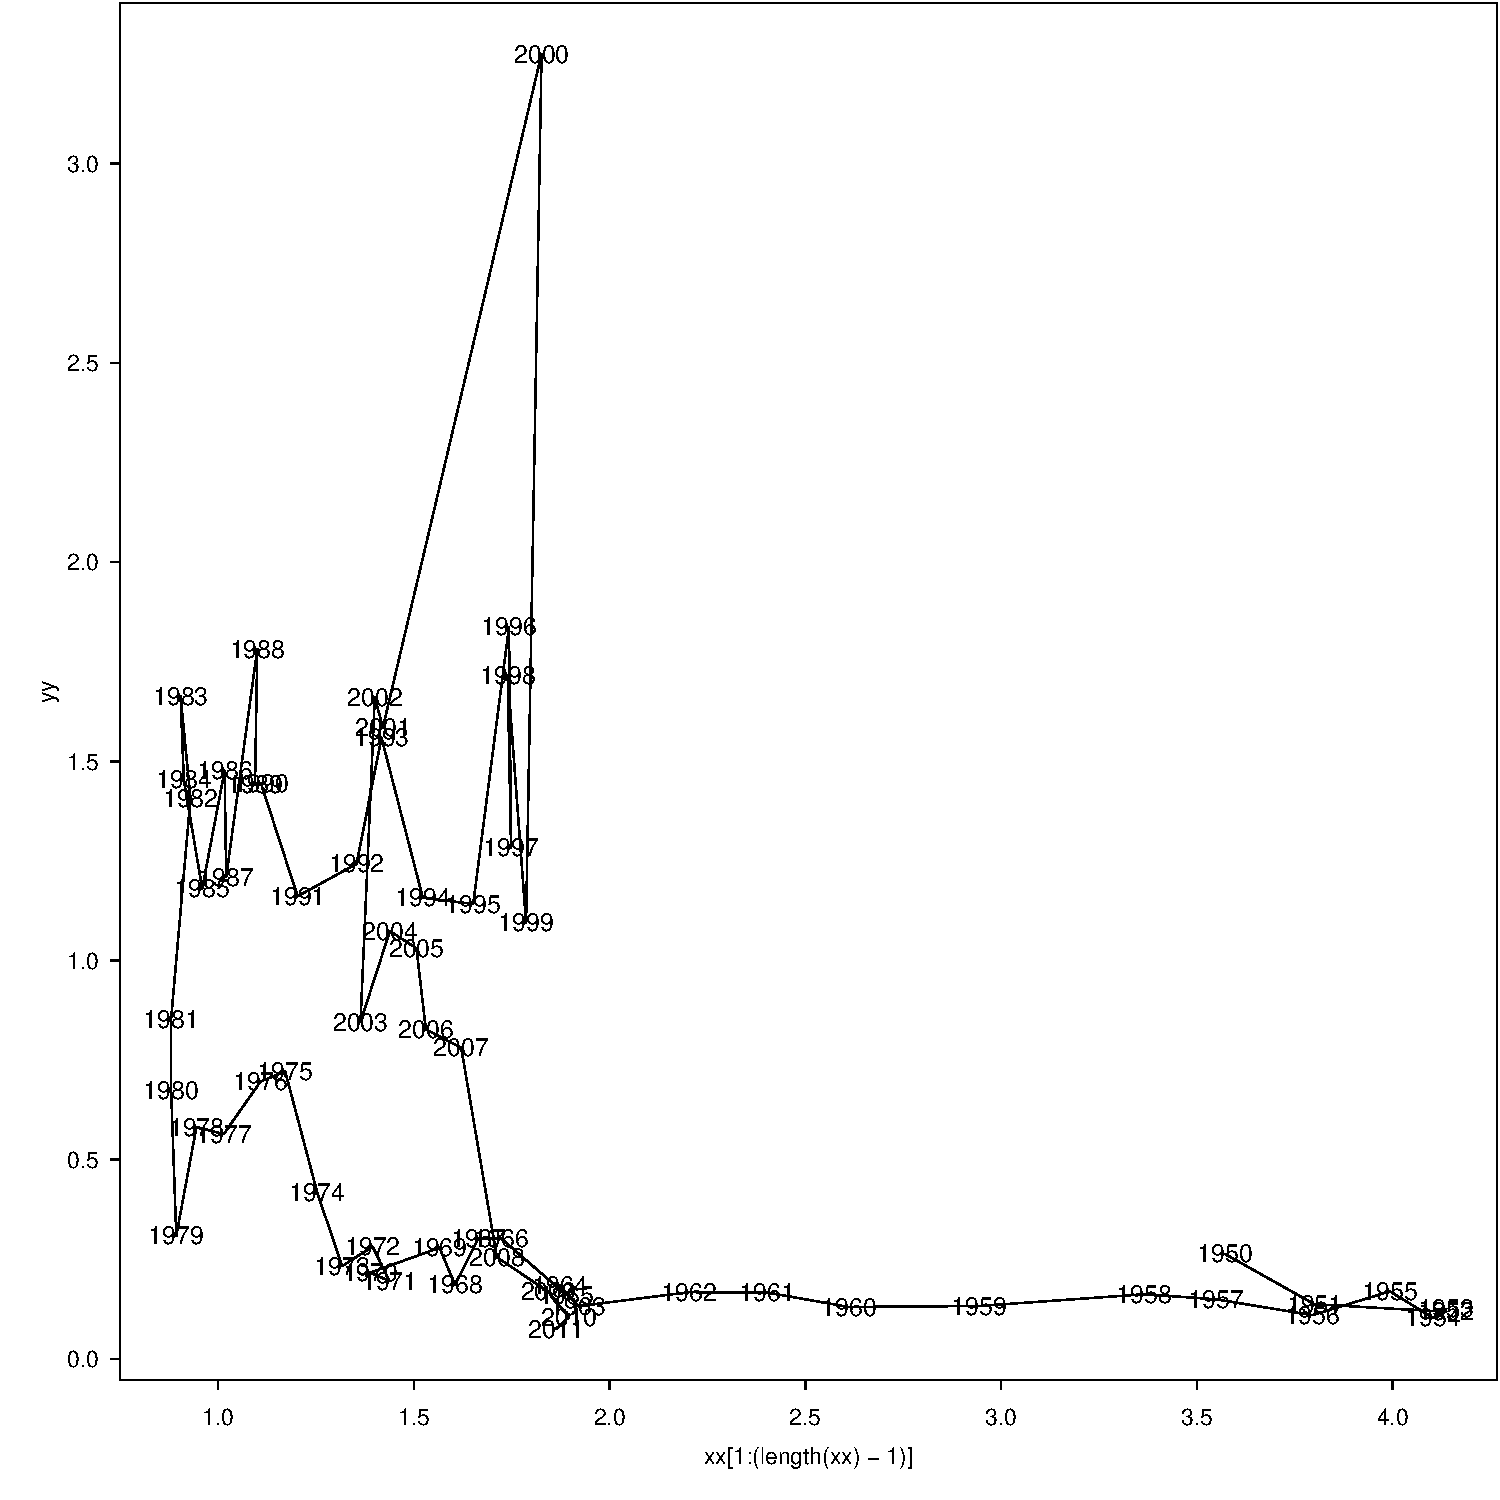
\includegraphics[width=.99\linewidth]{figure/minimal-boring-plots} 

}



\end{knitrout}


\section{Simulation tests}
\section{Stock assesment methodology}
\bibliographystyle{apalike}
\bibliography{biblio}

\end{document} 
